\documentclass[UTF8]{ctexart}
\usepackage{xcolor}
\usepackage{graphicx}
\usepackage[margin=1.5in]{geometry}
\usepackage{float}
\usepackage{listings} 
\usepackage{fancyhdr} %用于调整页眉的样式
\usepackage{fancyvrb} 
\usepackage{tabularx}


\title{Week 1}
\author{左昊天}
\date{\today}

\pagestyle{fancy}
\fancyhead[L]{ }
\setlength{\headheight}{27pt}


\lstset{
    numbers=left,
    numberstyle=\tiny,
    frame=shadowbox,
    rulesepcolor= \color{ red!20!green!20!blue!20},
    escapeinside=``,
    xleftmargin=2em,aboveskip=1em,
    framexleftmargin=2em,
    breaklines=true
}

\begin{document}

\maketitle

\section{Latex}

\subsection{章节}
章节:\verb|\section{}|

子章节:\verb|\subsection{}|

三级章节:\verb|\subsubsection{}|

\subsection{加粗}\verb|\textbf{}|
\subsection{斜体italic}
\verb|\textit{}|  
 
\textcolor{red}{注:中文的斜体和英文的斜体样式不一样}

例:\textit{中文样式}\qquad\textit{English version}

\subsection{下划线}\verb|\underline{}|

\subsection{添加图片及其标题} 
\subsubsection{添加图片} 
先引入graphicx包,再用\verb|\includegraphics{此处填图片的地址}| 
\subsubsection{添加标题} 
先将图片放在figure中,再在图片的下面加\verb|\caption{}|
例:

\begin{figure}[H]
    \centering
    
\includegraphics[width=0.2\textwidth]{photo.jpg}
    \caption{举例}
\end{figure}

\textbf{遇到的问题:}
\bigskip

(1)添加图片后,不显示图片

原因:图片过大导致无法显示

解决办法:通过\verb|
\includegraphics[width=0.2\textwidth]{photo.jpg}|等比例设置图片的宽高。
\bigskip

(2)图片出现在了章节前面。

原因:figure是浮动体,系统会自动决定浮动体的放置位置

解决办法:加入宏包\verb|\usepackage{float}|,并在\verb|\begin{figure}|后加上[H]属性,强制控制浮动位置。即\verb|\begin{figure}[H]|


\subsection{改变文字颜色} 
加入宏包\verb|\usepackage{xcolor}|,使用 \verb|\textcolor{color}{想输入的文字}| 控制颜色。

\subsection{列表} 
\subsubsection{无序列表} 
\textbf{代码:}
\begin{lstlisting}
    \begin{itemize}
        \item
        \item
    \end{itemize}
\end{lstlisting}
\qquad \textbf{例:}
\begin{itemize}
    \item 项1
    \item 项2
\end{itemize}

\subsubsection{有序列表} 
\textbf{代码:}
\begin{lstlisting}
    \begin{enumerate}
        \item
        \item
    \end{enumerate}
    \end{lstlisting}
\qquad \textbf{例:}
\begin{enumerate}
    \item 项1
    \item 项2
\end{enumerate}

\subsection{表格} 
\begin{lstlisting}
    \begin{tabular}{|p{3cm}|c|c|}
        \hline
        单元格1 & 单元格2 & 单元格3 \\
        \hline  \hline
        单元格4 & 单元格5 & 单元格6 \\
        \hline
        单元格7 & 单元格8 & 单元格9 \\
        \hline
    \end{tabular}
\end{lstlisting}
\begin{tabular}{|p{3cm}|c|c|}
    \hline
    单元格1 & 单元格2 & 单元格3 \\
    \hline  \hline
    单元格4 & 单元格5 & 单元格6 \\
    \hline
    单元格7 & 单元格8 & 单元格9 \\
    \hline
\end{tabular}\bigskip

\textbf{解释:}\\
1.\verb|p{3cm}|设置列宽\\
2.\verb|\hline|加横线\\
3.|p\verb|{|3cm\verb|}|c|c|中的c表示该列居中对齐(centering)



\subsection{公式}
\subsubsection{行内公式}
代码:\verb|$此处填写公式$|

例:$F=ma$ , $E=mc^2$
\subsubsection{单独一行的公式}
有两种写法:

\textbf{写法一:}
\begin{lstlisting}
    \begin{equation}
        此处填写公式
    \end{equation}
\end{lstlisting}
\qquad 例:
\begin{equation}
    F=ma
\end{equation}

\textbf{写法二:}
\begin{lstlisting}
    \[
        此处填写公式
    \]
\end{lstlisting}
\qquad 例:
\[
    E=mc^2
\]

\subsection{如何在latex中展示代码} 
\subsubsection{行内代码} 
\begin{lstlisting}
  \verb|此处填入代码|
\end{lstlisting}

\subsubsection{代码块} 
\begin{Verbatim}
    \begin{lstlisting}
        此处填写代码
    \end{lstlisting}
\end{Verbatim}

\newpage
\section{Git}
\subsection{查看文件状态}
\subsubsection{文件状态}
\begin{table}[H]
    \centering
    \begin{tabular}{|c|c|c|c|}
        \hline
        Untrack & Unmodified & Modified & Staged\\
        未跟踪 & 未修改 & 已修改 & 已暂存\\
        \hline
    \end{tabular}
\end{table}
\subsubsection{查看文件状态}
\verb|git status 文件名|\quad 用于查看单个文件的状态\par
\verb|git status| 可查看当前文件夹所有文件的状态\par
也可使用通配符,如: git status *.tex \\
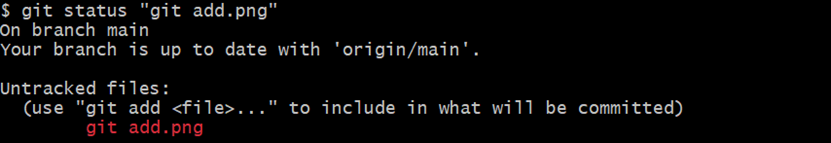
\includegraphics[width=1\textwidth]{status1.png}\\
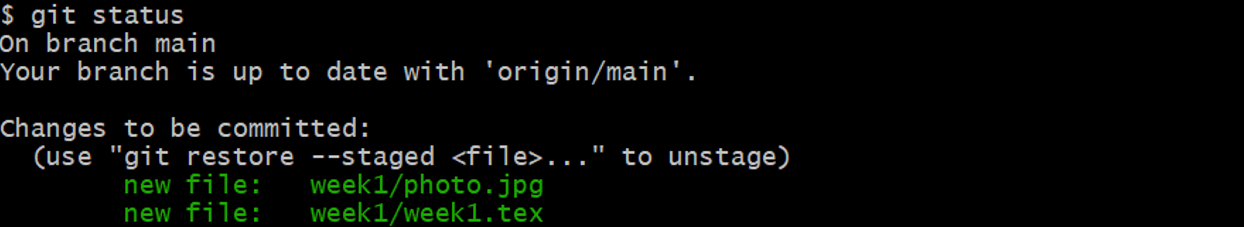
\includegraphics[width=1\textwidth]{status2.png}

\subsection{添加和提交文件}
\subsubsection{将文件添加到暂存区}

\verb|git add 文件名| \quad 添加单个文件\par 
\verb|git add .| 可将当前文件夹的所有文件添加到暂存区\par
也可使用通配符\par
补充:\verb|git rm --cached 文件名| \quad 可以将文件取消暂存\\
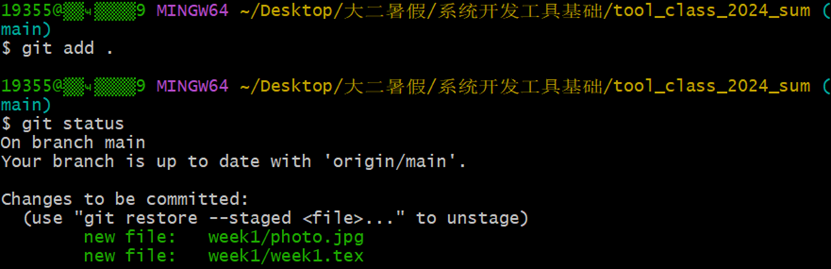
\includegraphics[width=1\textwidth]{git add.png}
\subsubsection{将暂存区的文件提交到本地仓库}
\verb|git commit -m "提交的信息"| \quad 将暂存区的文件提交到本地仓库\\
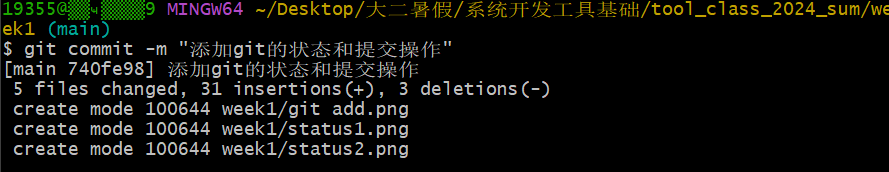
\includegraphics[width=1\textwidth]{commit1.png}\par
注意:如果不加 -m "提交的信息",git会进入vim编辑器,让你添加提交的信息。\\
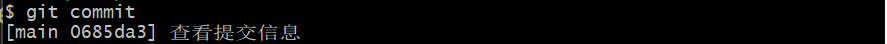
\includegraphics[width=1\textwidth]{commit2-1.png}\\
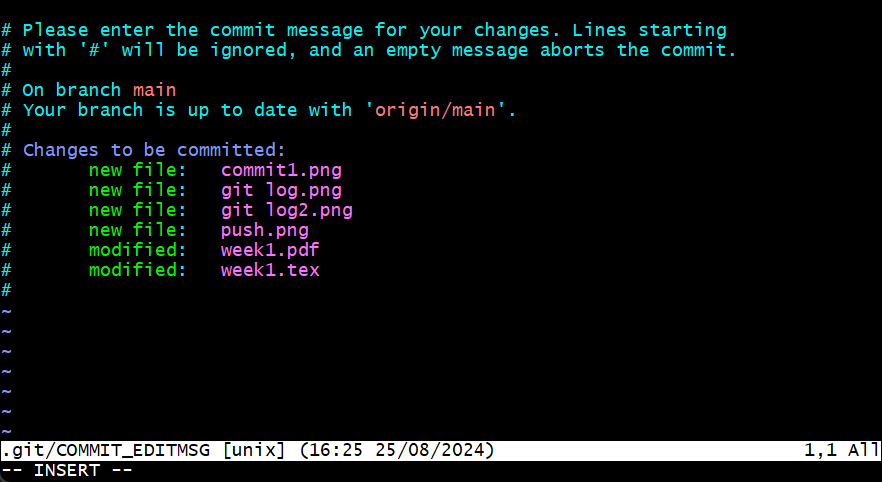
\includegraphics[width=1\textwidth]{commit2-2.png}\par

\subsection{查看提交信息}
\verb|git log| \quad 查看全部信息\par
\verb|git log --oneline| \quad 查看简要信息\\
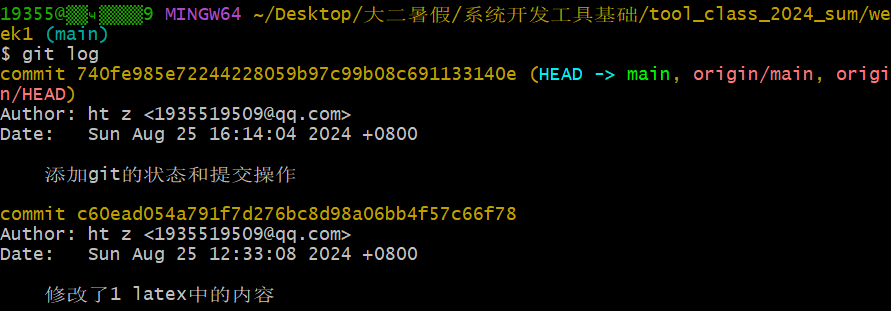
\includegraphics[width=1\textwidth]{git log.png}\\
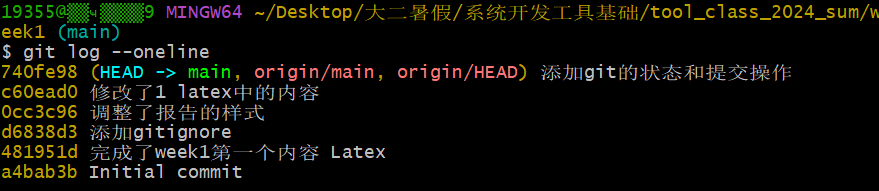
\includegraphics[width=1\textwidth]{git log2.png}

\subsection{远程仓库的相关操作}
\subsubsection{拉取}
\verb|git pull|\quad 将远程仓库的内容下载到本地仓库中
\subsubsection{推送}
\verb|git push|\quad 将本地仓库的内容上传到远程仓库\\
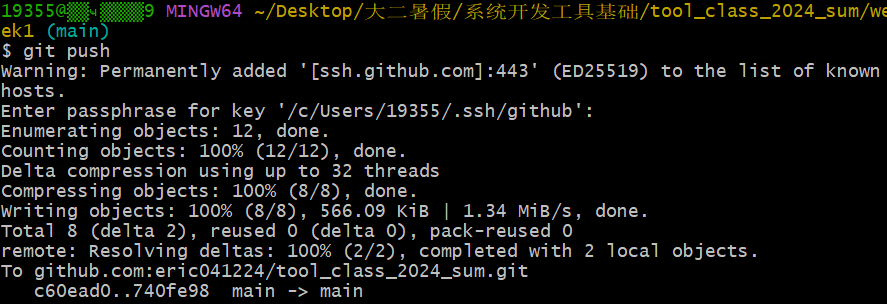
\includegraphics[width=1\textwidth]{push.png}

\subsection{查询所有操作的信息}
\verb|git reflog|\\
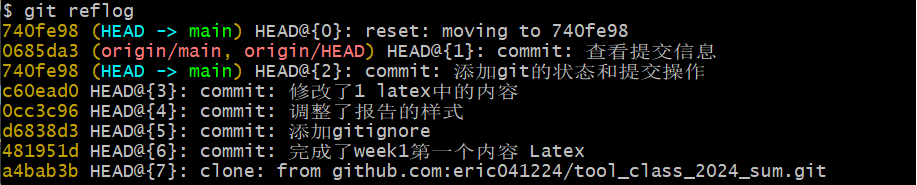
\includegraphics[width=1\textwidth]{reflog.png}\par
\textbf{可利用此功能撤销任意操作}
\subsection{版本回退}
版本回退有三种:\par
\begin{table}[H]
    \centering
    \begin{tabular}{|>{\centering\arraybackslash}p{3cm}|>{\centering\arraybackslash}p{1.5cm}|>{\centering\arraybackslash}p{1.5cm}|>{\centering\arraybackslash}p{5cm}|}
        \hline
        类型 & 工作区 & 暂存区 & 备注\\
        \hline
        git reset --soft & √ & √ & 回到指定版本,但此版本之后的文件依然存在,只是没提交\\
        \hline
        git reset --hard & × & × & 回到指定版本,此版本后的所有文件全部被删除\\
        \hline
        git reset --mixed & √ & × & 与soft类型的区别在于需要重新将文件添加到暂存区\\
        \hline
    \end{tabular}
\end{table}
其中,√表示此区域的文件不会被删除,×表示此区域的文件会被删除。\par
并且类型后面需要加上版本ID。
\subsection{查看差异}
\verb|git diff|\quad 默认展示工作区和暂存区的差异\par
\verb|git diff HAED|\quad 展示工作区与仓库的差异\par
\verb|git diff --cached|\quad 展示暂存区与仓库的差异\par
\verb|git diff 版本ID1 版本ID2|\quad 展示两个版本之间的差异\par
\textbf{注:在这些命令后加上文件名,那么就只展示这个文件的差异}
\subsection{删除文件}
将暂存的文件从工作区删除后,需要git add 的命令\par
也可使用git rm直接同时删除工作区和暂存区的文件\par
\textbf{但必须提交才能删除仓库的文件}
\end{document}
